\subsection{模型假设}

\begin{enumerate}[(1)]
    \item 假设电视台有多个频道,且各频道定位清晰,目标受众有显著差异;
    \item 假设电视台同频道不同时段的节目观众组成大致相同,即同频道不同节目的目标受众分类特征的差异可忽略;
    \item 假设买方对制作的广告定位清晰,且对广告的评估合理;
    \item 假设电视台对其受众的分析精准,能调查了解主要受众的基本信息;
    \item 为简化匹配过程,假设电视频道和视频广告的目标用户分类特征一致.
\end{enumerate}

\subsection{模型建立}

\subsubsection{确定分类特征}

搜集相关资料,我们得知,商业广告在投放时考虑的受众的主要特征如下:

\begin{enumerate}[(1)]
    \item 受众的基本个人信息,如年龄、性别、职业等,这有利于商品精准定位目标受众群体;
    \item 受众的购买力状况,可直接向用户调查了解收入状况,也可通过职业加以判断;
    \item 用户的偏好和收视习惯,可通过获取用户的历史收视和购买记录来获取.
\end{enumerate}

根据假设,电视频道和视频广告的目标用户分类特征一致,
因此再结合以上分析可以考虑将二者的分类特征划分为:

\begin{itemize}
    \item 年龄:依据少年、青年、中年、中老年、老年五个年龄阶段分别以1~5进行表示;
    \item 性别:1代表男性,2代表女性,3代表目标受众无性别上的差异;
    \item 购买力:依据用户的消费能力由低到高由1~5之间的整数表示;
    \item 受教育程度:根据用户的文化程度按小学、初中、普通高中、大专、大专及以上分别以1~5的整数表示;
    \item 消费意愿:根据用户倾向于消费的程度由低到高由1~5之间的整数表示;
    \item 情感倾向:根据用户喜好的情感的表达倾向按理性和感性两级从1~5进行分级.
\end{itemize}

\subsubsection{主成分分析}

以上本文给出了一个将用户分类特征划分为六个属性的示例,
但在实际的分析中模型更为复杂,在数据维数过高的情况下,
一些噪声数据对结果存在较大影响,且模型求解的效率较低.
因此本文为提取变量信息,减少分析的维度,使问题变得更简单、直观,
引入主成分分析的方法来简化模型.其基本步骤如下:

\begin{enumerate}[(1)]
    \item 对所给各项指标进行标准化处理
    \begin{equation}
        Z_{ij}=\frac{x_{ij}-\overline{x_j}}{s_j},(i=1,2,…,n;j=1,2,…,p),
    \end{equation}
    其中,
    \begin{equation}
        \overline{x_j}=\frac{1}{n}\sum\limits_{i=1}^{n}x_{ij},s_j^2=\frac{1}{n-1}
        \sum\limits_{i=1}^{n}(x_{ij}-\overline{x_j})^2(j=1,2,…,p)
    \end{equation}
    \item 根据标准化后的数据矩阵求出相关系数矩阵 $R$
    \begin{equation}
        R=\begin{pmatrix}
        r_{11} & r_{12} & \cdots & r_{1p}\\
        r_{21} & r_{22} & \cdots & r_{2p}\\
        \vdots & \vdots & \ddots & \vdots\\
        r_{n1} & r_{n2} & \cdots & r_{nn}\\
        \end{pmatrix},
    \end{equation}
    其中$r_{ij}(i=1,2,…,n;j=1,2,…,p)$为原变量 $x_i$ 与 $y_j$ 之间的相关系数,其计算公式为
    \begin{equation}
        r_{ij}=\frac{\sum\limits_{k=1}^{n}(x_{ki}-\overline{x_i})(x_{kj}-\overline{x_j})}{\sqrt{\sum\limits_{k=1}^{n}(x_{ki}-\overline{x_i})^2\sum\limits_{k=1}^{n}(x_{kj}-\overline{x_j})^2}}
    \end{equation}
    \item 求出相关系数矩阵 $R$ 的特征根 $\lambda$ 和特征向量 $l$
    \\首先解特征方程$\left| \lambda I-R\right|=0$,可用雅可比法(Jacobi)求出特征值$\lambda_i(i=1,2,\cdots,p)$,并使其按大小顺序排列,$\lambda_1\geq\lambda_2\geq\cdots\geq\lambda_p\geq0$;然后分别求出对应于特征值$\lambda_i$的特征向量$e_i(i=1,2,\cdots,p)$.这里求$\left\|e_i\right\|=1$,即$\sum\limits_{J=1}^{p}e_{ij}^2=1$,其中 $e_{ij}$ 表示向量 $e_i$ 的第 $j$ 个分量.
    \item 计算主成分贡献率及累计贡献率
    \\主成分 $z_i$ 的贡献率:
    \begin{equation}
        \frac{\lambda_i}{\sum\limits_{i=1}^{p}\lambda_i} (i=1,2,\cdots,p)
    \end{equation}
    累计贡献率:
    \begin{equation}
        \frac{\sum\limits_{k=1}^{i}\lambda_i}{\sum\limits_{k=1}^{p}\lambda_i}(i=1,2,\cdots,p)
    \end{equation}
    \item 确定主成分 $F_1,F_2,…,F_k$
    \\一般取累计贡献率达到$85\%-95\%$的特征值 $\lambda_1,\lambda_2,\cdots,\lambda_m$ 所对应的第1,第2,…,第$m(m \leq p)$个主成分 $F_1,F_2,…,F_k$.
\end{enumerate}

\subsubsection{快速聚类($K$均值聚类)}

聚类是研究对样品或指标进行分类的一种多元统计方法,
是一句研究对象的个体的特征进行分类的方法.
聚类分析把分类对象按一定规则分成若干类,这些类非事先给定的,
而是根据某种特征确定的.在同一类中这些对象在某种意义上趋向于彼此相似,
而在不同类中趋向于不相似.

上文中提到了使用主成分分析的方法确定 $p$ 个指标来表示电视频道用户特征,
根据模型假设,本文使用同样的指标来表示视频广告目标用户的用户特征.
接下来,本文通过电视台的频道总数确定一个$K$值,
对买方提供的视频广告进行K均值聚类分析.其基本的过程如下:

\begin{enumerate}[(1)]
    \item 数据无量纲化
    \\由于数据之间的量纲不相同,不便于比较.因此需要对数据进行0-1规格化,即将数据统一放到0~1的范围,将其转化为无量纲的纯数值,便于不同单位或量级的指标能够进行比较和加权.简记特征向量为$A$,则
    \begin{equation}
        v_i'=\frac{v_i-\min(A)}{\max{(A)}-\min{(A)}},v_i\in A    
    \end{equation}
    \item 随机选取 $k$ 个中心点
    \\ 随机选取训练数据中的 $k$ 个点作为起始中心点.
    \item 遍历所有数据,将每个数据划分到最近的中心点中
    \\ 每个样本都有 $p$ 个指标,因此每个样本可以看成 $p$ 维空间中的一个点,可以用距离来度量样本间的接近程度.常用的距离的算法有绝对距离、欧式距离、切比雪夫距离、明考斯基距离.
    \\本文采用欧式距离,即用
    \begin{equation}
        d_{ij}=\sqrt{\sum\limits_{t=1}^{p}(x_{it}-x_{jt})^2}    
    \end{equation}
    来刻画样本 $X_i$ 与 $X_j$ 之间的距离.
\end{enumerate}

\subsubsection{匹配与推送}

上文中,我们得到了广告的 $K$ 个分类,以下简称为广告簇.
可以计算得出各个广告簇的中心向量 $\bm{\alpha_i} (i=1,2,\cdots,k)$,
电视频道用户画像的特征向量 $\bm{\beta_i} (i=1,2,\cdots,k)$
分别计算其两两之间的欧式距离
\begin{equation}
    d=\sqrt{\sum\limits_{t=1}^{p}(\bm\alpha_{it}-\bm\beta_{jt})^2},  
\end{equation}

其中,$i=1,2,\cdots,k;j=1,2,\cdots,k$
将所得结果记录在视频广告簇-电视频道用户(Advertisement-Channel)关联表中,以下简记为广告簇-频道关联表.

然后再根据关联度对广告簇和频道用户进行匹配,其思路如下:

\begin{enumerate}[(1)]
    \item 首先在广告簇-频道表中对应于广告簇的每一行的数据中找到该行的最小欧式距离,
    标记为待定值.
    \item 遍历表中每一行,若该行中的待定值为其所在列(对应于频道)中唯一的待定值,
    则将该值标记为确定值;
    \item 若该行中的待定值不是列中唯一的待定值,则找出这一列中的待定值中的最小值,
    则将该值改为确定值;
    对于该列中其它的待定值所在行,分别在对应未有确定值的列的数据中找到最小欧式距离,
    将该数据标记为确定值;
    \item 重复2,3步,直到表中的每一列和每一行都有且只有一个确定值,该确定值即
    广告簇和频道的一条匹配信息.
\end{enumerate}

最后根据匹配信息,对每个频道推送相应的广告簇

\subsection{模型求解}

针对本模型,本文编纂了以下数据进行求解与验证:

\begin{table}[H]
    \centering
    \caption{电视频道用户分类特征}
    \begin{tabular}{|l|c c c c c c|}
        \Xhline{1.2pt}
        \diagbox{频道}{特征} & 年龄 & 购买力 & 受教育程度 & 情感倾向 & 性别 & 消费意愿 \\
        \Xhline{1.2pt}
        少儿频道 & 1 & 2 & 2 & 5 & 3 & 3 \\
        体育频道 & 2 & 3 & 3 & 5 & 1 & 3 \\
        经济频道 & 3 & 5 & 5 & 1 & 3 & 4 \\
        法治频道 & 4 & 4 & 4 & 2 & 3 & 2 \\
        戏曲频道 & 5 & 1 & 2 & 4 & 2 & 2 \\
        \Xhline{1.2pt}
    \end{tabular}
    \label{tab:my_labe1}
\end{table}

使用SPSS统计分析软件的因子分析功能进行主成分分析,得到的结果如下:

\begin{figure}[H]
    \centering
    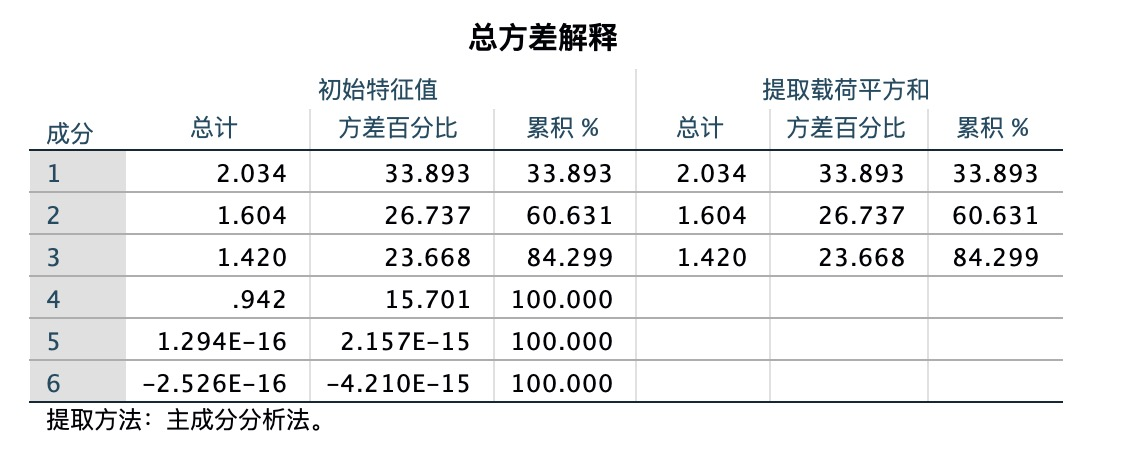
\includegraphics[scale=0.32]{resources/pic1.png}
    \caption{解的总方差}
    \label{pic1}
\end{figure}

根据以上结果,本文应当选取年龄、购买力、受教育程度作为主成分,但考虑到数据量过小导致结果不精确,
本文最终选取了年龄、购买力、受教育程度和情感倾向作为分类特征属性.

接下来,本文编纂了100条按以上述分类特征标记的广告信息,并通过SPSS软件进行快速聚类.聚类的结构如下:

\begin{figure}[H]
    \centering
    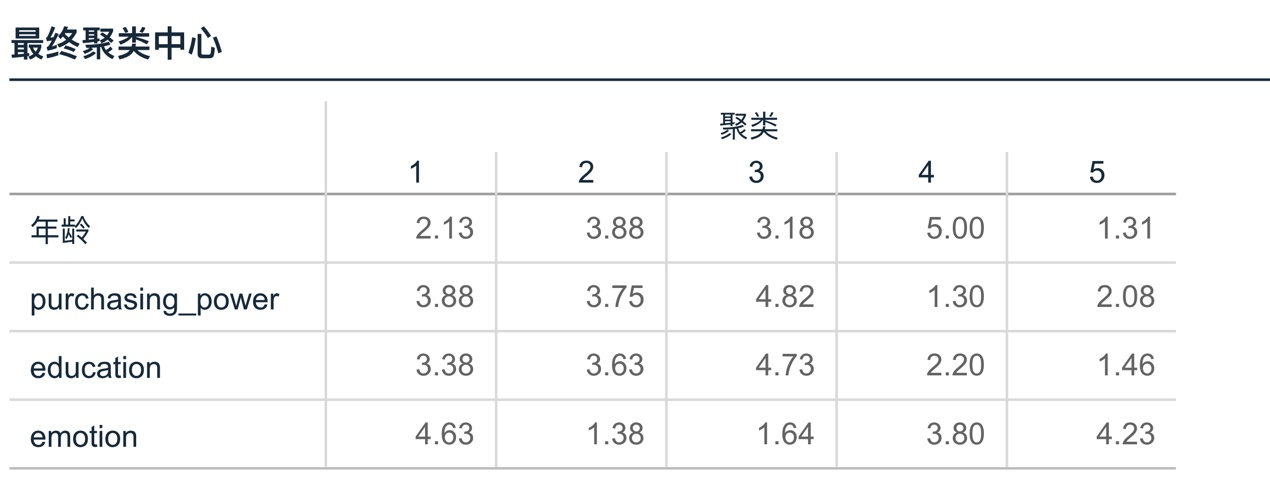
\includegraphics[scale=0.3]
        {resources/pic2.jpg}
    \caption{最终聚类中心}
    \label{pic2}
\end{figure}

对聚类中心和电视频道用户画像特征向量无量纲化并求解欧式距离,可解得:

\begin{table}[H]
    \centering
    \caption{视频广告簇-电视频道用户关联表}
    \begin{tabular}{|l|c c c c c|}
        \Xhline{1.2pt}
        \diagbox{广告簇}{频道} & 少儿频道 & 体育频道 & 经济频道 & 法治频道 & 戏曲频道 \\
        \Xhline{1.2pt}
        广告簇1 & 0.3393 & 0.1363 & 0.5595 & 0.4550 & 0.6157 \\
        广告簇2 & 0.8260 & 0.6206 & 0.2474 & 0.0766 & 0.6374 \\
        广告簇3 & 0.7950 & 0.5921 & 0.0952 & 0.1818 & 0.7631 \\
        广告簇4 & 0.6571 & 0.5481 & 0.7859 & 0.5462 & 0.0608 \\
        广告簇5 & 0.1244 & 0.1870 & 0.8320 & 0.6975 & 0.5964 \\
        \Xhline{1.2pt}
    \end{tabular}
    \label{tab:my_labe2}
\end{table}

根据以上结果,结合上述匹配算法,我们可以得到以下推送关系:

\begin{table}[H]
    \centering
    \caption{推送匹配关系表}
    \begin{tabular}{|c|c|}
        \Xhline{1.2pt}
        \textbf{广告簇} & \textbf{频道} \\
        \Xhline{1.2pt}
        广告簇1 & 体育频道 \\
        广告簇2 & 法治频道 \\
        广告簇3 & 经济频道 \\
        广告簇4 & 戏曲频道 \\
        广告簇5 & 少儿频道 \\
        \Xhline{1.2pt}
    \end{tabular}
    \label{tab:march}
\end{table}

\subsection{模型评价}

本模型的优点有

\begin{itemize}
    \item 本模型实现的方式较为简单,既可以通过编写代码进行匹配和推送,也可使用
    SPSS等统计分析软件对数据进行简单处理后进行匹配;
    \item 本模型实现的时间效率较高,主成分分析和K均值聚类算法均为线性的时间复杂度,
    而最后的匹配算法的时间复杂度为$O(n^2)$,其中 $n$ 为频道数;
\end{itemize}

本模型的缺点有

\begin{itemize}
    \item 本模型需要设定大量的特征分类特征之后,模型的匹配才能更加精确,而分类特征的设定是较耗时的,其拓展性较差;
    \item 本模型的分类特征的取值是人为设定的,存在较大的主观性和臆断性,且容易存在标准尺度不一的情况,对结果有较大影响;
    \item 本模型虽能处理小样本数据,但当广告个数与频道个数的比值过小时,广告特征聚类过于松散,推荐效果较差.
\end{itemize}
